\documentclass[11pt,a4paper]{article}
\usepackage[margin=2.2cm]{geometry}
\usepackage{tikz}
\usepackage{booktabs}
\usepackage{array}
\usepackage{float}
\usepackage{graphicx}
\usepackage{amsmath}
\usepackage[hidelinks]{hyperref}
\usetikzlibrary{arrows.meta,positioning,calc}
\graphicspath{{../../experiments/figures/}}

\title{Cyber Physical Robotics: Milestone 3\\
       \large Distributed Robot Control under Random Communication Delay}
\author{Code: \url{https://github.com/JaiPipatt/cpr-multi-robot-simulation}}
\date{}

\begin{document}
\maketitle
\vspace{-2.5em}

\section{Summary}
\textbf{Problem.} Every message now arrives after a random delay (exponential
distribution). Each robot receives the same message at a different step. The
Milestone 2 controller assumed all robots read messages at the same step, so it
fails in two ways:
\begin{enumerate}
\item \textbf{Two helpers for one goal.} Each robot chooses the closest helper from
the replies it has read so far. Robots read different replies, so several robots
think they are the closest and all walk to the goal.
\item \textbf{Picks at different times.} A robot picks when it receives
\texttt{READY} from its partner. The two \texttt{READY} messages arrive at
different steps, so one robot picks alone. This is an illegal pick.
\end{enumerate}

\textbf{Solution.} I separate two questions.
\begin{itemize}
\item \emph{Who} is the partner? This needs agreement between robots, so I use
\textbf{Paxos}. It works for any message delay.
\item \emph{When} to pick? Messages are not used. A robot picks when it
\emph{senses} exactly one other robot on its goal cell. Sensing has no delay, so
both robots pick in the same step.
\end{itemize}

\paragraph{Key message.}
\begin{itemize}
\item Paxos \textbf{guarantees exactly one partner} per goal, for any delay.
\item Paxos does \textbf{not} guarantee the \emph{nearest} partner. A nearer robot
may hear about the goal late, and the first valid proposal stays chosen.
\item The \textbf{backoff} makes the nearest robot \emph{likely} to propose first,
so it is likely to be chosen. Distance is used only for this; correctness does not
depend on it.
\end{itemize}
Safety comes from Paxos. A good choice comes from the backoff. The combination is
the contribution of this work.

\section{Messages}
A robot sends at most one broadcast per step (it may contain several payloads).
Each payload has the sender id and the sender's Lamport clock. A robot also
receives its own broadcast.

\medskip
\begin{tabular}{@{}lp{12.3cm}@{}}
\toprule
\textbf{Message} & \textbf{Content and purpose}\\
\midrule
\texttt{FOUND}    & Instance, goal id, goal position. Sent by the robot that finds a goal.\\
\texttt{PREPARE}  & Instance, ballot. Paxos phase 1a: a volunteer starts a round.\\
\texttt{PROMISE}  & Instance, addressee, ballot, last accepted ballot and value. Phase 1b.\\
\texttt{ACCEPT}   & Instance, ballot, value (partner id). Phase 2a.\\
\texttt{ACCEPTED} & Instance, ballot, value. Phase 2b, sent to all robots.\\
\texttt{PICKED}   & Goal id. Sent after a pick, so late messages about this goal are ignored.\\
\bottomrule
\end{tabular}

\medskip\noindent
An \emph{instance} is one announcement of a goal: (goal id, finder's Lamport
clock). If the finder times out, the goal is announced again as a new instance. A
\emph{ballot} is (Lamport clock, robot id), so two ballots are never equal.

\section{State machine}
\begin{figure}[H]
\centering
\resizebox{\linewidth}{!}{%
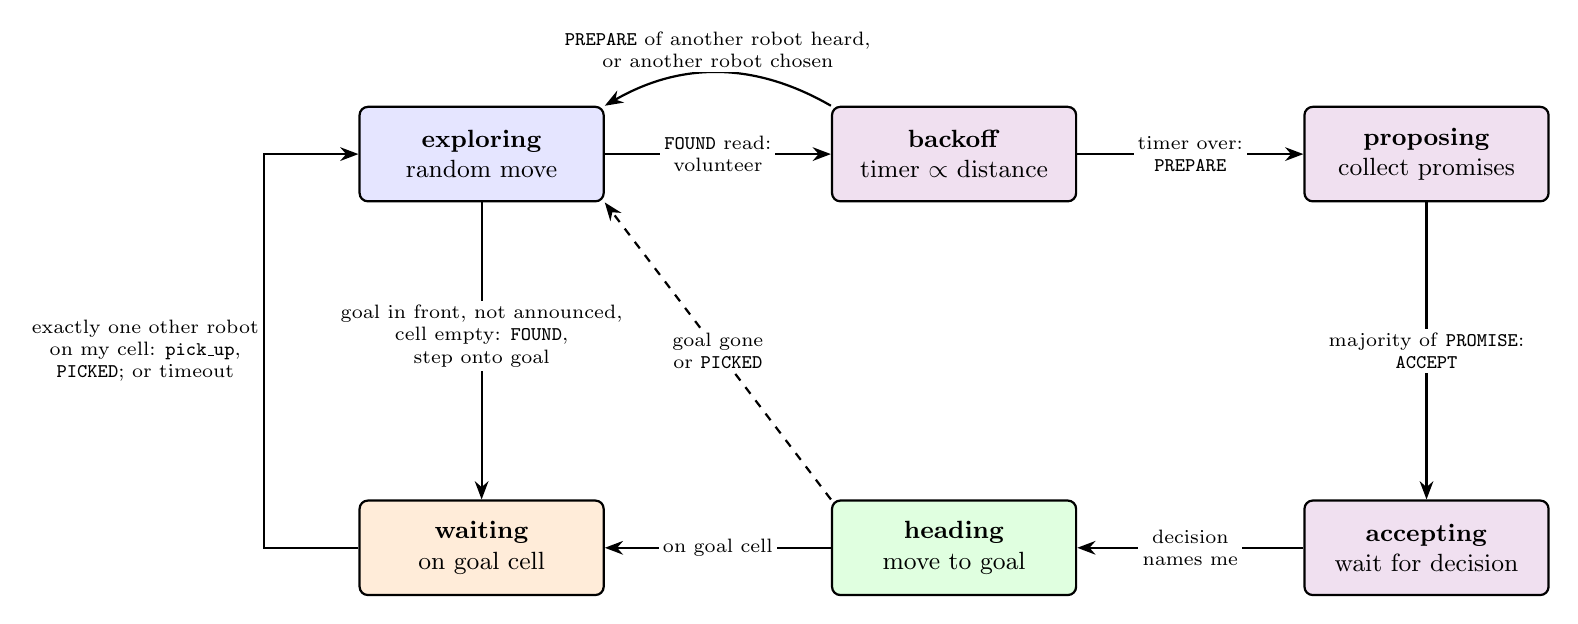
\begin{tikzpicture}[
    >=Stealth, thick,
    state/.style={draw, rounded corners=3pt, minimum width=3.1cm,
                  minimum height=1.2cm, align=center, font=\small},
    lbl/.style={font=\scriptsize, align=center, fill=white, inner sep=1.5pt}
]
\node[state, fill=blue!10]   (explore) at (0,0)     {\textbf{exploring}\\random move};
\node[state, fill=orange!15] (wait)    at (0,-5)    {\textbf{waiting}\\on goal cell};
\node[state, fill=violet!12] (back)    at (6,0)     {\textbf{backoff}\\timer $\propto$ distance};
\node[state, fill=violet!12] (prop)    at (12,0)    {\textbf{proposing}\\collect promises};
\node[state, fill=violet!12] (acc)     at (12,-5)   {\textbf{accepting}\\wait for decision};
\node[state, fill=green!12]  (head)    at (6,-5)    {\textbf{heading}\\move to goal};

\draw[->] (explore.south) -- node[lbl, pos=.45]{goal in front, not announced,\\cell empty: \texttt{FOUND},\\step onto goal} (wait.north);
\draw[->] (explore.east) -- node[lbl, pos=.5]{\texttt{FOUND} read:\\volunteer} (back.west);
\draw[->] (back.north west) to[out=150, in=30] node[lbl, above]{\texttt{PREPARE} of another robot heard,\\or another robot chosen} (explore.north east);
\draw[->] (back.east) -- node[lbl, pos=.5]{timer over:\\\texttt{PREPARE}} (prop.west);
\draw[->] (prop.south) -- node[lbl, pos=.5]{majority of \texttt{PROMISE}:\\\texttt{ACCEPT}} (acc.north);
\draw[->] (acc.west) -- node[lbl, pos=.5]{decision\\names me} (head.east);
\draw[->] (head.west) -- node[lbl, pos=.5]{on goal cell} (wait.east);
\draw[->, dashed] (head.north west) -- node[lbl, pos=.5]{goal gone\\or \texttt{PICKED}} (explore.south east);
\draw[->] (wait.west) -- ++(-1.2,0) |- node[lbl, pos=.25, left]{exactly one other robot\\on my cell: \texttt{pick\_up},\\\texttt{PICKED}; or timeout} (explore.west);
\end{tikzpicture}}
\caption{State machine of every robot. Not drawn: from \emph{proposing} and
\emph{accepting}, a robot goes to \emph{exploring} if the decision names another
robot, or to \emph{heading} if it names itself. In every state the robot is also a
Paxos acceptor and learner.}
\end{figure}

\section{States}\label{sec:states}
\begin{description}
\item[exploring] Random moves; never steps onto a goal cell. If it senses an
unannounced goal in front and the cell is empty, it sends \texttt{FOUND}, steps on
the goal and goes to \emph{waiting} (it is the \emph{finder}). If it reads a
\texttt{FOUND} for an undecided instance and an unpicked goal, it volunteers for
the closest such goal and goes to \emph{backoff}.

\item[backoff] The volunteer waits as many steps as its Manhattan distance to the
goal. At step $t$, with robot position $(x_r,y_r)$ and goal position $(x_g,y_g)$:
\[
  d = |x_r - x_g| + |y_r - y_g|, \qquad t_{\text{backoff}} = t + d .
\]
The robot leaves \emph{backoff} at the first step $t' \ge t_{\text{backoff}}$.
A closer robot waits less, so it usually proposes first. If it hears a
\texttt{PREPARE} for the same instance while waiting, another robot is already
handling the goal, and it returns to \emph{exploring}. Otherwise it makes a ballot,
sends \texttt{PREPARE} and goes to \emph{proposing}.

\item[proposing] Collects \texttt{PROMISE} replies. With a majority (more than
$N/2$ robots) it sends \texttt{ACCEPT}. The value is its own id, unless a promise
reports an already accepted value; then it must use the value with the highest
accepted ballot.

\item[accepting] Waits for the decision. If the decision is its own id, it is the
partner and goes to \emph{heading}; otherwise it returns to \emph{exploring}.

\item[heading] Moves to the goal (x first, then y). Before entering the cell it
senses that the goal is still there and that at most one robot stands on it.
Then it goes to \emph{waiting}.

\item[waiting] Stands on the goal cell. When it senses exactly one other robot on
the cell, it does \texttt{pick\_up} and sends \texttt{PICKED}. If nobody comes in
60 steps, it gives up and returns to \emph{exploring}.
\end{description}

\section{Why Paxos gives one partner}
Every robot is an \emph{acceptor} and a \emph{learner}. A volunteer is also a
\emph{proposer}. An acceptor keeps, per instance, the highest ballot it promised
and the last ballot and value it accepted. It promises only to a higher ballot. It
accepts an \texttt{ACCEPT} only if it has not promised a higher ballot. A learner
decides when a majority reports \texttt{ACCEPTED} for the same ballot.

\paragraph{One partner.} Any two majorities share at least one robot. After a
value is accepted by a majority, every later proposer collects promises from a
majority, so at least one promise reports that value, and the proposer must
propose the same value again. A late robot with a higher ballot cannot install a
different partner. The argument has no timing assumption, so it holds for any
delay.

\paragraph{Not necessarily the nearest.} For the same reason, the first chosen
partner stays chosen even if a nearer robot proposes later. Example from a
simulator run: robot 7 was chosen with ballot (2,\,7). The \texttt{FOUND} reached
robot 4 late, so robot 4 proposed with the higher ballot (59,\,4). The promises
reported ``accepted value 7'', so robot 4 had to send \texttt{ACCEPT} with value 7.
The decision did not change. The backoff reduces how often this happens, because
far robots wait longer before they propose.

\section{Why picks are legal}
A robot picks only when it is on its goal cell and senses exactly one other robot
there. Both robots sense each other in the same step, so both pick in the same
step. For ``exactly one other robot'' to mean ``my partner'', entry to a goal cell
is controlled:
\begin{itemize}
\item a finder steps onto a goal only if the cell is empty;
\item exploring robots never step onto a goal cell;
\item the partner enters only if the goal is still there and at most one robot
stands on it;
\item every robot remembers picked goals and ignores late messages about them.
\end{itemize}

\section{Simulation results}\label{sec:results}
\paragraph{Setup.} 10$\times$10 grid, 8 robots, 10 goals spawned whenever all goals
are gone. Each message delay is drawn per receiver from an exponential distribution
with the given mean, rounded down to whole steps. For each mean delay and each
controller I ran 20 seeds of 2000 steps. The Milestone 2 controller is the
Milestone 2 submission, run in the same environment.

\begin{figure}[H]
\centering
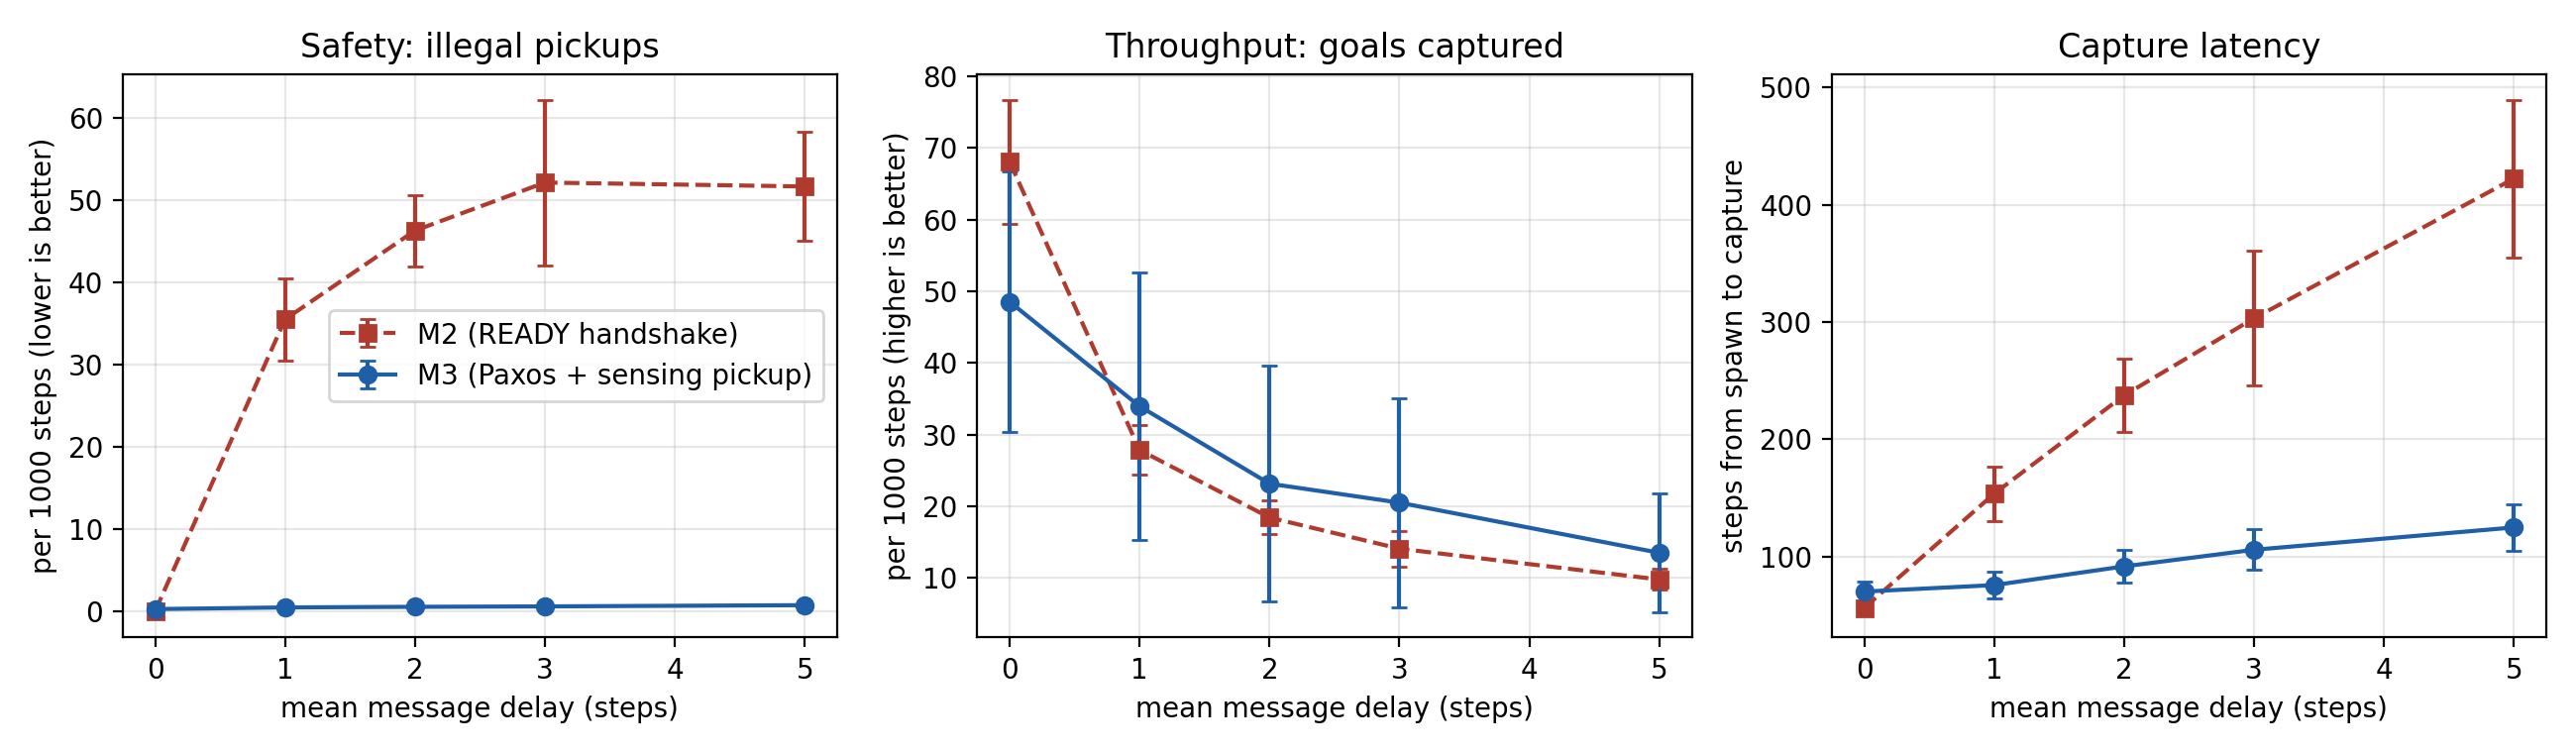
\includegraphics[width=\linewidth]{m2_vs_m3.png}
\caption{Milestone 2 vs Milestone 3. Mean and standard deviation over 20 runs.}
\end{figure}

\begin{table}[H]
\centering
\begin{tabular}{@{}r rr rr rr@{}}
\toprule
& \multicolumn{2}{c}{Illegal picks / 1000 steps} & \multicolumn{2}{c}{Captures / 1000 steps} & \multicolumn{2}{c}{Capture latency (steps)}\\
\cmidrule(lr){2-3}\cmidrule(lr){4-5}\cmidrule(l){6-7}
Mean delay & M2 & M3 & M2 & M3 & M2 & M3\\
\midrule
0 & 0.00 & 0.25 & 68.0 & 48.5 & 56 & 70\\
1 & 35.52 & 0.45 & 27.9 & 34.0 & 154 & 76\\
2 & 46.33 & 0.53 & 18.4 & 23.1 & 237 & 92\\
3 & 52.17 & 0.57 & 14.1 & 20.5 & 303 & 106\\
5 & 51.70 & 0.72 & 9.8 & 13.5 & 422 & 125\\
\bottomrule
\end{tabular}
\caption{Values behind the figure (8 robots, 20 runs of 2000 steps per cell).}
\end{table}

\begin{itemize}
\item \textbf{Safety.} With delay, M2 makes 36 to 52 illegal picks per 1000 steps.
M3 makes 0.45 to 0.72, about 99\% fewer. Of the 101 illegal picks in M3 runs, 99
were path crossing: a robot heading to a different goal walked over a waiting
finder. In no run did two robots learn different partners for one instance.
\item \textbf{Throughput.} At delay 0, M2 captures more, because M3 pays for the
backoff and two Paxos round trips. With any delay, M3 captures more.
\item \textbf{Latency.} From delay 0 to 5, M3 latency grows from 70 to 125 steps.
M2 latency grows from 56 to 422 steps.
\end{itemize}

\section{Scalability}
Paxos needs a majority, so with 100 robots a proposer needs 51 replies. I varied
the number of robots from 4 to 128 at mean delays 1, 3 and 5 (5 runs of 800 steps).
\emph{Paxos time} is the time from the first \texttt{PREPARE} of an instance until
the chosen partner learns the decision. \emph{Deliveries} count every payload
received by every robot.

\begin{figure}[H]
\centering
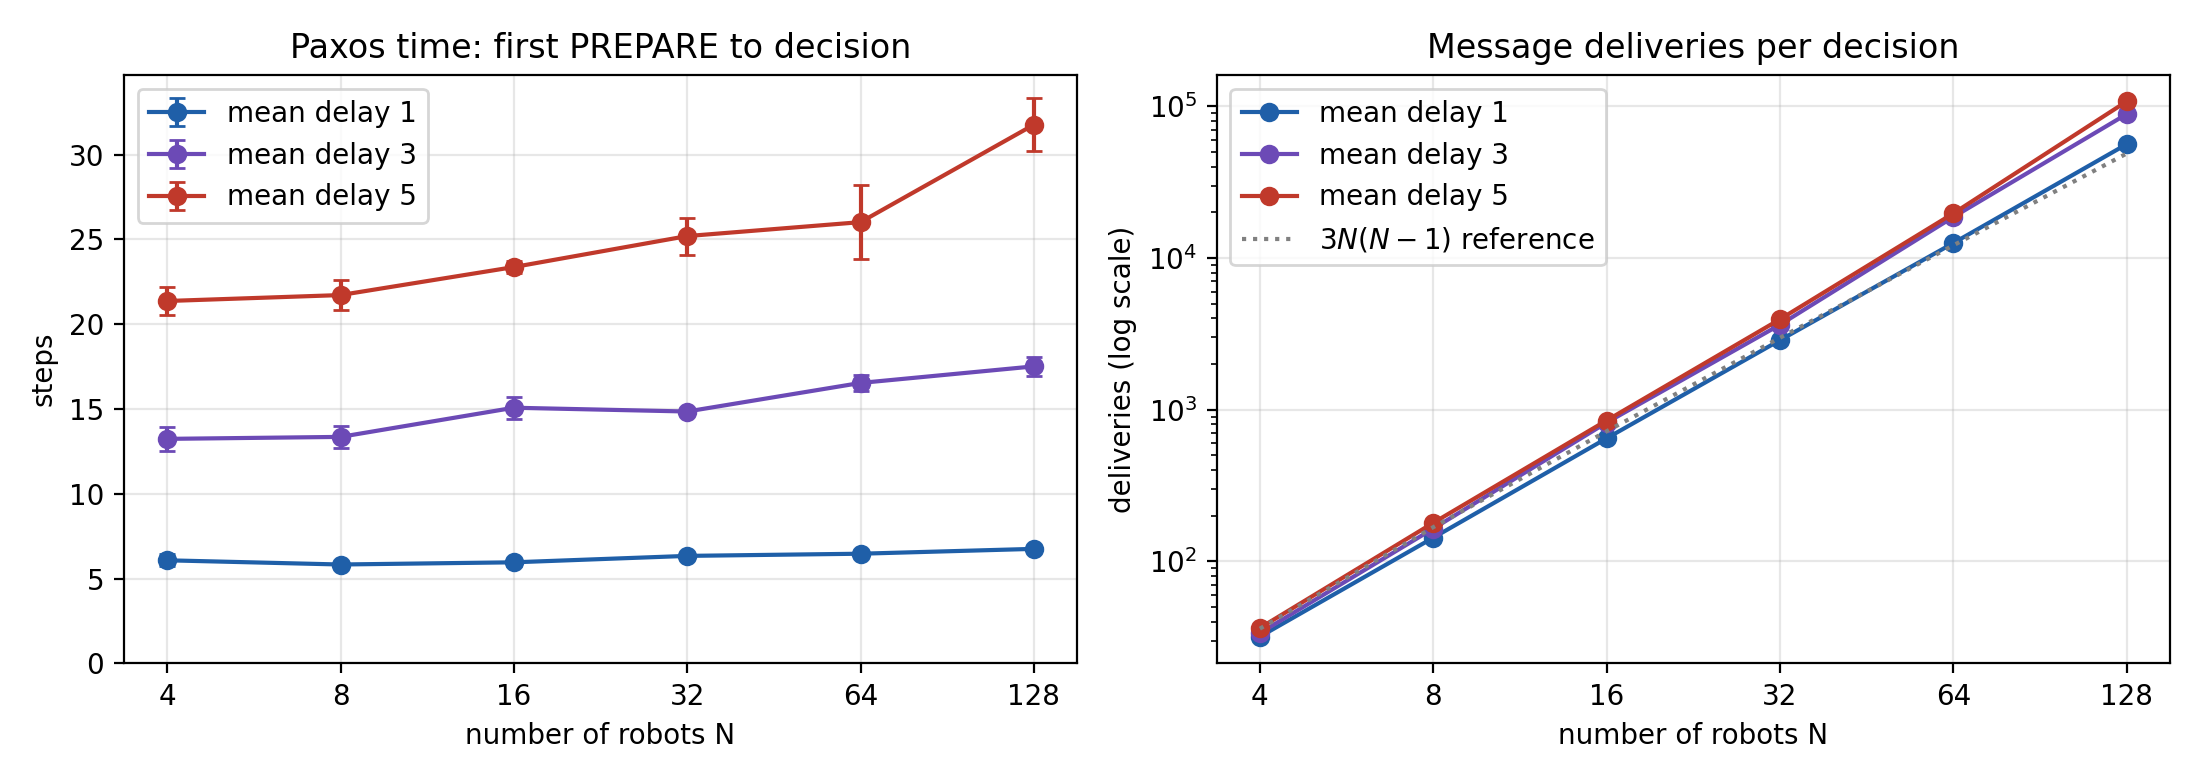
\includegraphics[width=\linewidth]{scaling.png}
\caption{Paxos time and message cost as the number of robots grows.}
\end{figure}

\begin{itemize}
\item \textbf{Time grows slowly.} A proposer waits for the \emph{fastest} majority,
not the slowest robot. The time until half of the replies arrive is close to the
median delay, which does not depend on $N$. At mean delay 1, Paxos time goes from
6.1 to 6.8 steps (4 to 128 robots). At mean delay 5, from 21.4 to 31.8 steps,
because with many robots several volunteers have almost the same backoff, so more
rounds compete.
\item \textbf{Messages grow quadratically.} Every robot answers every
\texttt{PREPARE} and \texttt{ACCEPT}, and every answer goes to all $N$ robots. One
decision costs about $2N(N-1)$ deliveries, plus competing rounds: 32 at 4 robots,
about 56\,000 at 128 robots (mean delay 1). The cost of scale is network load, not
waiting time. Two possible fixes, not implemented: use a small fixed group of
acceptors (for example 5), which makes the cost linear in $N$; or split the grid
into regions with one Paxos group each.
\end{itemize}

\section{Timeout}\label{sec:limits}
The waiting timeout (60 steps) is fixed and does not adapt to the delay. At large
delays some pairs give up before their partner arrives, and the goal is announced
again. This costs throughput but not safety.

\end{document}
